%!TEX root=report.tex
\subsection{k-means clustering}
\label{section:result-kmeans}

\subsubsection{Indentifing the amount of clusters}
Due to the size of the dataset (64800, 341), and the fact multiple simulated datasets of the same size would be needed to calculate the gap-statistic it was calculated on the HPC cluster that DTU offers for students and faculty.
It should be noted that if such a setup had not been available, one could have used smaller subsamples of the data.
20 simulation samples of size (64800,341) were made using a multivariate uniform distribution. The following is the plot of the resulting gap statistic with its standard deviation.
\begin{figure}[H]
	\center
	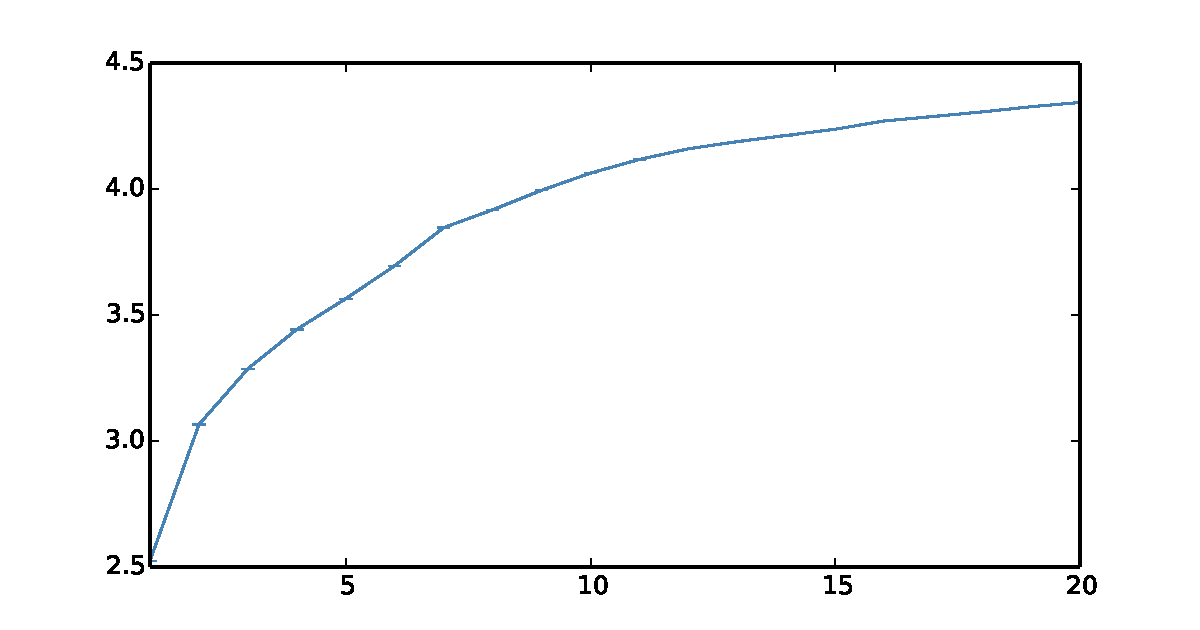
\includegraphics[width=\textwidth]{figures/kmeans-gap}
	\caption{Gap-statistics with standard deviation. Note the standard deviation is very small.}
	\label{fig:kmeans-gap}
\end{figure}

From Figure \ref{fig:kmeans-gap} it is seen that according to the gap-statistics the optimal amount of cluster, is more than 20. Unfortunately such a high number of clusters are not suitable for visualization. Instead 7 clusters have been chosen; this is based on the large slope change which can be observed in the gap-statistics graph. This is also seems like a suitable number of colors for visualization.

\begin{figure}[H]
	\center
	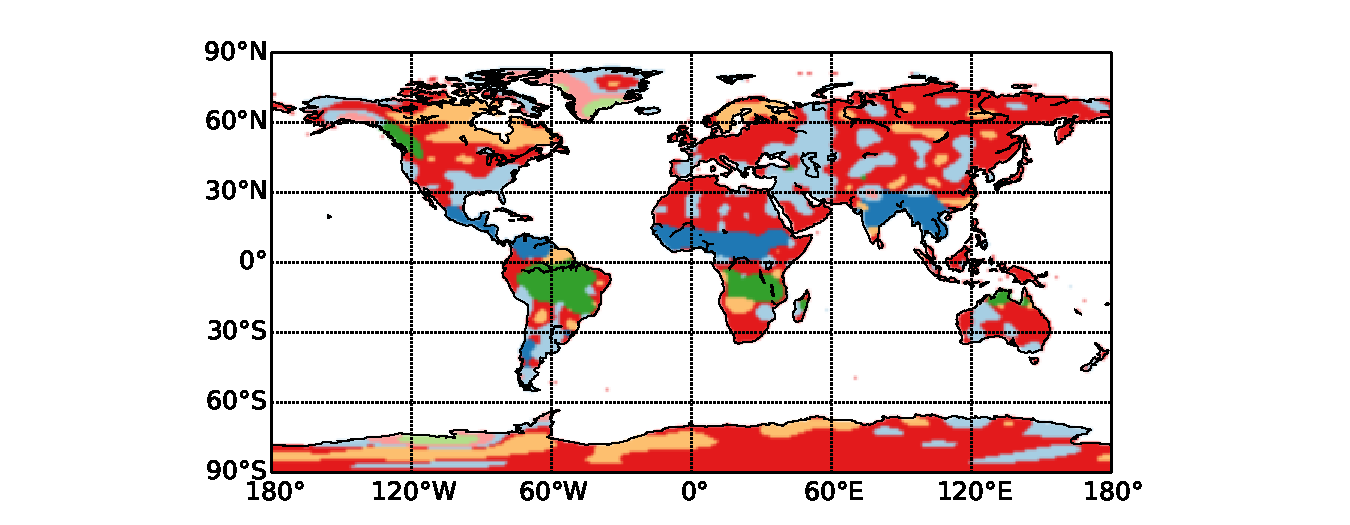
\includegraphics[width=\textwidth]{figures/kmeans-world}
	\caption{Each position is an point with belongs to the cluster, with the closest centroid.}
	\label{fig:kmeans-world}
\end{figure}
\begin{figure}[H]
	\center
	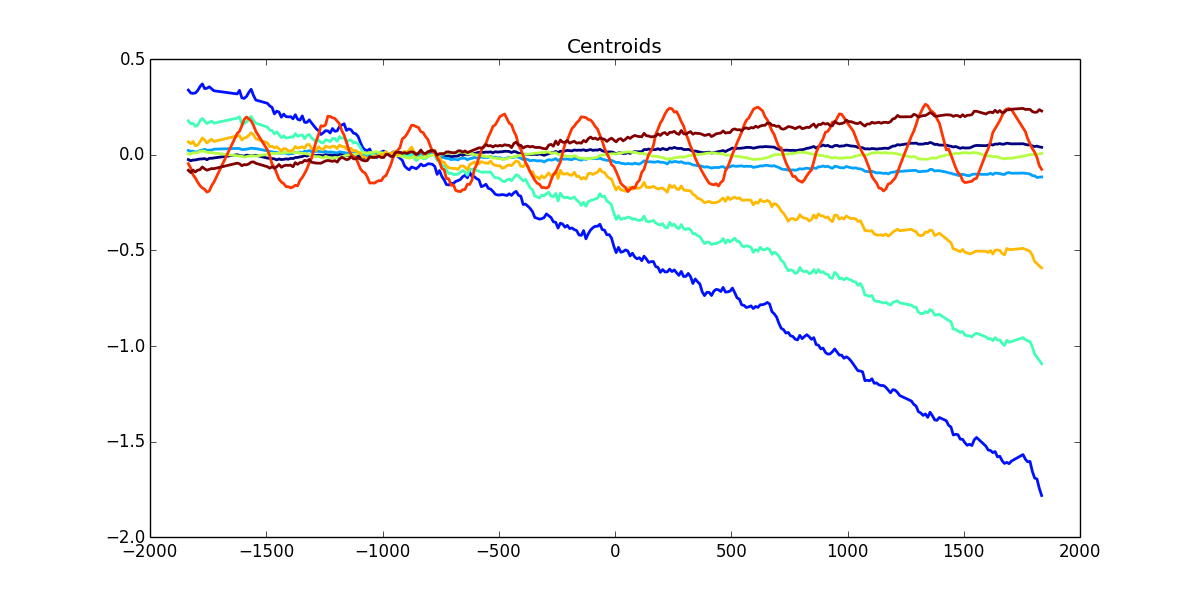
\includegraphics[width=\textwidth]{figures/kmeans-centroids}
	\caption{Cluster centroids. The colors correspond to those in Figure \ref{fig:kmeans-world}}
	\label{fig:kmeans-centroids}
\end{figure}

Comparing the two plots above a few interesting insights are gained:
\begin{itemize}
	\item Orange areas have a slight mass increase. At the south pole it appears that some of the mass loss at the edge actually moves inward towards the South Pole. This may be caused by post glacial rebound as no GIA has been performed.
	\item  Green and blue correlates with extreme and regular seasonality (i.e. rain season in Amazon Basin).
	\item Light green and pink correspond with trending mass loss. The most significant locations appear to be located around the tip of the Western Antarctica along with Greenland's east coast.
\end{itemize}
